%%%%%%%%%%%%%%%%%%%%%%%%%%%%%%%%%%%%%%%%%%%%%%%%%%%%%%%%%%%%%%%%%%%%%%%%%%%%%%%%
%%  Article LaTeX style, by Anthony Wharton
\documentclass[11pt,twocolumn,a4paper]{article}
\usepackage[backend=bibtex,style=numeric-comp,sorting=none]{biblatex}
\usepackage[compact]{titlesec}
\usepackage{geometry}
\usepackage{lipsum}
\usepackage{listings}
\usepackage{graphicx}
\usepackage{xspace}
\usepackage{textcomp}
\usepackage{array}
\usepackage{caption}
\usepackage{titling}
\usepackage{calc}
\usepackage{setspace}
\usepackage{changepage}

%%%%%%%%%%%%%%%%%%%%%%%%%%%%%%%%%%%%%%%%%%%%%%%%%%%%%%%%%%%%%%%%%%%%%%%%%%%%%%%%
%%  Package Setup

% Set up borders and column separation
\setlength{\columnsep}{0.7cm}
\geometry{left=1.2cm,right=1.2cm,top=1cm,bottom=1.2cm}

% Set up title spacing
% \titlespacing{command}{left spacing}{before spacing}{after spacing}[right]
\titlespacing\section{0pt}{1pt}{1pt}
\titlespacing\subsection{0pt}{1pt}{1pt}
\titlespacing\subsubsection{0pt}{1pt}{1pt}


% Set up paragraph spacing and enforce hyphenation penalty
\setlength{\parindent}{0.7em}
\setlength{\parskip}{0.5em}
\setlength{\textfloatsep}{0.25cm}
\setlength{\droptitle}{-1.3cm}
\setlength{\footskip}{\paperheight
    -(2cm+\voffset+\topmargin+\headheight+\headsep+\textheight)
    -1.2cm}
\hyphenpenalty 500

% Set up figure/table captions
% \DeclareCaptionLabelSeparator{emdash}{\textemdash}
\DeclareCaptionFont{mysize}{\fontsize{9}{9.6}\selectfont}
\captionsetup{font=mysize,justification=centering}

% Set up bibliography
\bibliography{references}
\renewcommand*{\bibfont}{\small}

% Set up more intelligent trademark symbol with spacing
% \let\OldTexttrademark\texttrademark
% \renewcommand{\texttrademark}{\OldTexttrademark\xspace}
\def\tm{\texttrademark\xspace}

% Set up code appropriate code listing appearance.
\lstset{
    basicstyle=\footnotesize,
    % numbers=left,
    % numberstyle=\tiny,
    xleftmargin=1.2em,
    columns=flexible,
    linewidth=\columnwidth,
    breaklines=true,
    captionpos=b,
    escapeinside=\!\!,
    language=C,
    literate={->}{$\rightarrow{}$}{1}
             {=>}{$\Rightarrow{}$}{1},
    moredelim=[is][\ttfamily\kern-0.1ex\textsubscript]{^}{\ },
    morekeywords={}
}

% \begin{lstlisting}[gobble=8, caption="A sample code listing.", label=lst1]

\begin{document}
%%%%%%%%%%%%%%%%%%%%%%%%%%%%%%%%%%%%%%%%%%%%%%%%%%%%%%%%%%%%%%%%%%%%%%%%%%%%%%%%
%%  Title
\title{\LARGE\bfseries Exploring Jacobi Method Parallelism}
\date{\vspace{-1cm}} % No date
\author{Anthony Wharton \\ aw15885@bristol.ac.uk}
\maketitle

%%%%%%%%%%%%%%%%%%%%%%%%%%%%%%%%%%%%%%%%%%%%%%%%%%%%%%%%%%%%%%%%%%%%%%%%%%%%%%%%
%%  Abstract
\begin{abstract}
After exploring optimisations within a sequential implementation of the Jacobi method, this report continues further, exploring the performance benefits of moving to a parallel solution.
\end{abstract}


%%%%%%%%%%%%%%%%%%%%%%%%%%%%%%%%%%%%%%%%%%%%%%%%%%%%%%%%%%%%%%%%%%%%%%%%%%%%%%%%
%%
\section{Initial Sequential Solution}
The last coursework saw many optimisations explored to the serial version of the Jacobi method. It is assumed that this has been read, however not necessary. This report serves an a continuation from the last report. In that report effective memory management and vectorisation brought the best performance gains, with focus on the loading to and saving from the cache. \par

The final run times for this serial code is:

\begin{figure}[h]
        \centering
        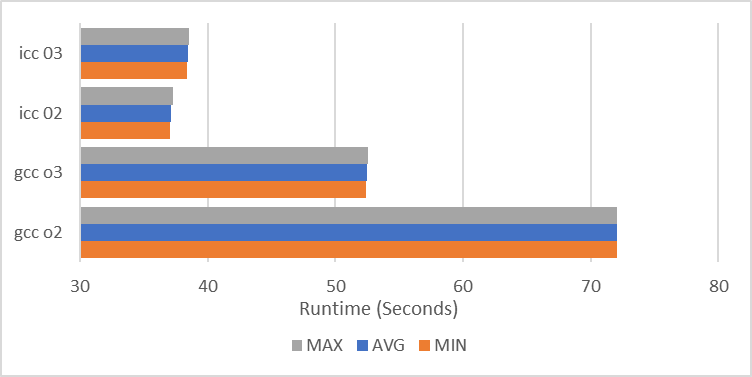
\includegraphics[width=0.8\linewidth]{figures/1-SEQ.png}
        \caption{Times achieved for $4000\times4000$ with the original serial code on various compilers. Min, Avg. and Max figures were taken from 10 repeated runs of the code.}
        \label{fig-1-seq}
\end{figure}

For this report, timings after different optimisations will be graphed for the different compilers and their configurations at $4000\times4000$. This enables the ability to see how the algorithm performs with less variance from thread overhead as would be seen with smaller boards, yet minimises the required run time to get the results. All graphs will include a minimum, average and maximum time figure, taken from 10 repeats of the code at that point. It should also be noted that order to simplify the process of adding OpenMP pragma's later in the report, the serial code which used \texttt{static inline} functions was flattened into just one function - something that had no performance hit. \par


%%%%%%%%%%%%%%%%%%%%%%%%%%%%%%%%%%%%%%%%%%%%%%%%%%%%%%%%%%%%%%%%%%%%%%%%%%%%%%%%
%%
\section{Approaching the Problem}
As was discovered previously, the majority of computation within the Jacobi method was within the matrix dot products. Currently in the serial method, this is within a double nested for loop. Each iteration of the outer loop is distinct, in that they require no dependency on other iterations in order to be computed. This makes the problem embarassingly parallelizable as different iterations of the loop can be distributed amongst different workers. \par


%%%%%%%%%%%%%%%%%%%%%%%%%%%%%%%%%%%%%%%%%%%%%%%%%%%%%%%%%%%%%%%%%%%%%%%%%%%%%%%%
%%
\section{OpenMP and Optimisations}
Given the knowledge that this outer \texttt{for} loop is in fact embarassingly parallelizable, OpenMP can be introduced very trivially. OpenMP is a API that allows for multiprocessing amongst different platforms and languages. Within the context of the code for this report, which is written in C, this is implemented with the addition of a compiler flag to enable OpenMP and pragma's to control it. There are also some environment variable and API functions, however the majority of control comes from the pragma's.

\subsection{Parallel For}
The first step in parallelizing the code is to add one of the most fundamental and basic pragma's offered by OpenMP; \texttt{\#pragma omp parallel for} above the line declaring the outer for loop. The \texttt{parallel} keyword states that a team of threads should be created to execute the next control block in a parallel manner. The \texttt{for} keyword more specifically states that the iterations of the following loop should be run in the established team of threads. \par

As already stated, there is no dependance with the dot product operations meaning this is perfectly valid. However, the convergence checking does require some inter-iteration dependency. Thus the difference measure code was moved out of the for loop into it's own sequential loop that runs after the parallel for loop that deals with the calculation. This will be addresses in due course, but running the preceeding solution greatly reduces the time this method takes from upwards of 70 seconds in the case of \texttt{gcc -o2} (Figure \ref{fig-1-seq}) to below 20 seconds in most cases for all the compilers (Figure \ref{fig-2-omp}). The 29 second run with \texttt{gcc -o2} appeared to be an outlier, but for integrity was not ommited. \par

\begin{figure}[h]
        \centering
        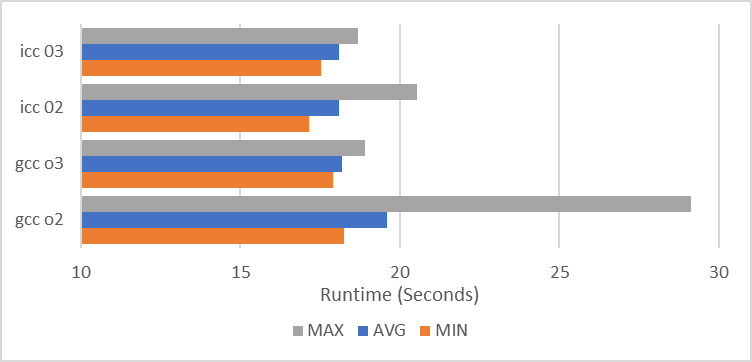
\includegraphics[width=0.8\linewidth]{figures/2-OMP-OUTER.png}
        \caption{Times achieved for $4000\times4000$ after adding the \texttt{\#pragma omp parallel for}.}
        \label{fig-2-omp}
\end{figure}


\subsection{Reduction}
In the last section, there was the slight hiccup of having to remove the difference measure from the main calculation loop. This leaves two loops, one for the main calculation and the other for calculating the difference measure. As the difference measure is far less computationally expensive, it could be left as it is. However, for the purpose of academic experimentation it would be beneficial to try and see if this can be improved upon. The first attempt to do this was to parallelize the second loop, however this has neglibable difference and in some cases was slower. The cost of initialising a team of threads to the relitively simple computation here is not worth it. \par

With the failure of naive parallelism, the \texttt{reduction} keyword is introduced to the original main loop pragma. OpenMP provides a \textit{'design pattern'} of sorts for the common problem of shared accumulators for teams of threads. This keyword instructs threads to do partial reduction operations on the chosen accumulator when they have completed. These partial reductions eventually get collated into the final end value in a tree like fasion dependant on the finish time of the thread. The partial reductions are done with initial values that make sense to the reduction opeation chosen, and not the user provided initial value for the accumulator. This allows the threads to work privately and only collate the results later in execution time. \par

In this case, the reduction is done with \texttt{+:sqdiff} and merges the two loops back together again. This addition beared little difference to the timing results, one again most probably due to the simplistic computation.

\begin{figure}[h]
        \centering
        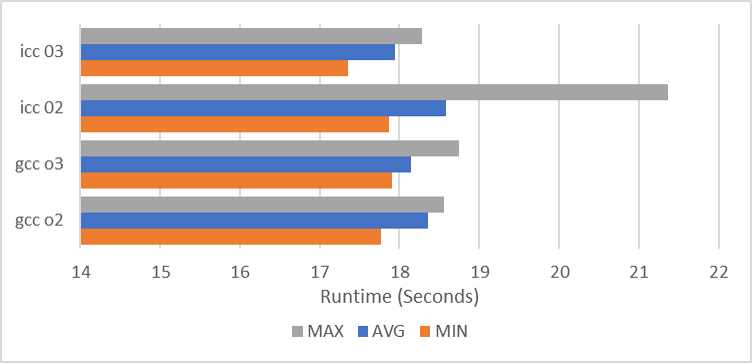
\includegraphics[width=0.8\linewidth]{figures/3-INNER-REDUX.png}
        \caption{Times achieved for $4000\times4000$ after introducting the \texttt{reduction} keyword for \texttt{sqdiff}.}
        \label{fig-3-redux}
\end{figure}


\subsection{Single Instruction, Multiple Data}
In the last report vectorisation was a prevelant topic. Not only were options within the compiler explored, but also manual help was given in explicitly calculating multiple rows at once with very verbose code. This ensured that cache thrashing was minimal and cache lines were being loaded optimally. OpenMP also adds support for single instruction, multiple data (SIMD) - i.e. vectorisation. \par

This is a much more portable option as the implementation will deal with how the vectorisation is carried out in the compiler - a key goal of OpenMP. With this enabled, it allows for the removal of the very long, verbose \& explicit multiple row calculations from the implementation. This not only makes the code far more readable but also will fix any old bugs where problem sizes that are not divisible by 8 (the number of rows being calculated at once) would break for free. However, unsurprisingly as vectorisation was heavily explored previously this once again has little tangiable effect on the run time. \par

\begin{figure}[h]
        \centering
        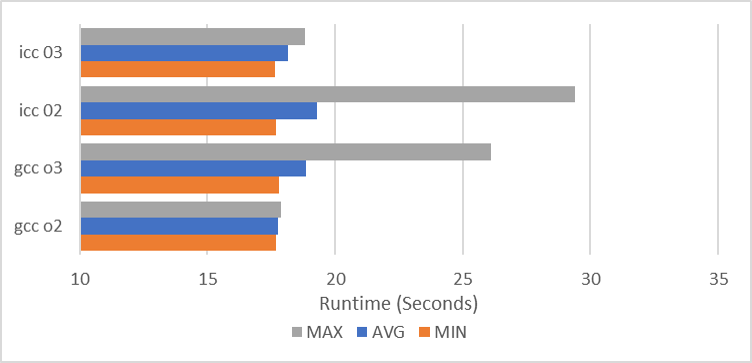
\includegraphics[width=0.8\linewidth]{figures/4-SIMD-W-REDUX.png}
        \caption{Times achieved for $4000\times4000$ after introducting the \texttt{reduction} keyword for \texttt{sqdiff}.}
        \label{fig-3-redux}
\end{figure}


%%%%%%%%%%%%%%%%%%%%%%%%%%%%%%%%%%%%%%%%%%%%%%%%%%%%%%%%%%%%%%%%%%%%%%%%%%%%%%%%
%%
\section{Memory Alignment}



%%%%%%%%%%%%%%%%%%%%%%%%%%%%%%%%%%%%%%%%%%%%%%%%%%%%%%%%%%%%%%%%%%%%%%%%%%%%%%%%
%%
\section{CPU Affinity}



%%%%%%%%%%%%%%%%%%%%%%%%%%%%%%%%%%%%%%%%%%%%%%%%%%%%%%%%%%%%%%%%%%%%%%%%%%%%%%%%
%%  Conclusion
\vspace{-0.1cm}
\section{Conclusion}


\vspace{-0.2cm}
\begin{table}[h]
\begin{adjustwidth}{-0.15cm}{}
\small
\centering
\begin{tabular}{c|c|c|c}
    & \textbf{1000$\times$1000} & \textbf{2000$\times$2000} & \textbf{4000$\times$4000}   \\
\textbf{\texttt{orig.}} & 10.895/10.878 & 131.856/131.760 & 1031.428/1030.911 \\
\textbf{\texttt{opt.}} & 0.365/0.355 & 2.632/2.593 & 38.655/38.500 \\
\textbf{\texttt{\% inc.}} & $2985\%$ & $5001\%$ & $2668\%$ \\
\end{tabular}
\caption{}
\label{finalResults}
\end{adjustwidth}
\end{table}\par
\vspace{-0.22cm}

%%%%%%%%%%%%%%%%%%%%%%%%%%%%%%%%%%%%%%%%%%%%%%%%%%%%%%%%%%%%%%%%%%%%%%%%%%%%%%%%
%%  Bibliography
\vspace{-0.3cm}
\printbibliography[title={Bibliography}]
\end{document}

% \begin{figure}[h]
%     \includegraphics[width=18em]{Figures/twoLayers.pdf}
%     \centering
%     \caption{Two Layers to be composed together.}
%     \label{twolayers}
% \end{figure}
